\chapter{Spectral submanifolds and model reduction}
We now outline a dynamical systems approach to model reduction. Our goal is to identify globally attracting invariant sets $S$ and understand the reduced dynamics on said sets, i.e. to find the reduced order model. However, we must address the issue of the existence, uniqueness, and smoothness of these sets. Smoothness is not a given, as attractors are very often not smooth manifolds, as seen in Fig. \ref{fig:nonsmooth_set}.
\begin{figure}[h!]
	\centering
	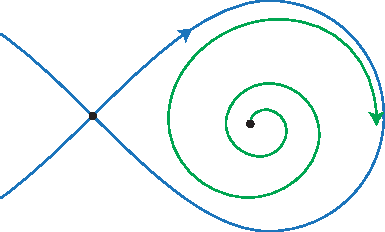
\includegraphics[width=0.4\textwidth]{figures/ch9/27nonsmooth_set.pdf}
	\caption{An example of a globally attracting set which is not a smooth manifold.}
	\label{fig:nonsmooth_set}
\end{figure}

In order to study these objects, we must first set out a few definitions.
\begin{definition}
	The \emph{global attractor} is the largest bounded, invariant, set (in forward and backward time) that attracts trajectories.
\end{definition}
\begin{definition}
An \emph{inertial manifold} is a manifold of lower dimension than the full ambient space, that is attracting, forward-invariant manifold that is at least Lipschitz and contains the global attractor.
\end{definition}

The existence of inertial manifolds is not guaranteed in general, however the following proposition provides a sufficient condition \cite{FoiasInertial}.
\begin{proposition}[] \label{prop:FoiasExistence}
	If we have the dynamical system defined on a Hilbert space $H$
	\begin{align}
		\dot{u} = Au + R(u,u);\quad u\in H.
	\end{align}
Then given the following conditions:
\begin{enumerate}
	\item $A$ is self-adjoint, negative definite, and densely defined;
	\item $A^{-1}$ is compact;
	\item $R(u,u)$ is bilinear and is suitably dominated in norm by $Au$;
\end{enumerate}
then we have that the following hold:
\begin{enumerate}
	\item All trajectories enter a ball $B$ at some point;
	\item The timit set of the whole ball is the global attractor (inside the ball);
	\item An inertial manifold $M$ exists.
\end{enumerate}
Such a global attractor within a ball $B$ and the inertial manifold $M$ is depicted in Fig. \ref{fig:FoiaProp}.
\end{proposition}
\begin{figure}[h!]
	\centering
	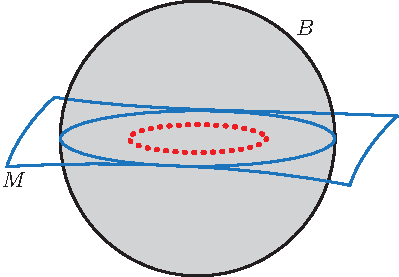
\includegraphics[width=0.4\textwidth]{figures/ch9/28FoiaProp.pdf}
	\caption{The red global attractor contained within the ball $B$ and the inertial manifold $M$ in the case of proposition \ref{prop:FoiasExistence}.}
	\label{fig:FoiaProp}
\end{figure}

An example in which such an $M$ is proven to exist can be found in the reaction-diffusion equation
\begin{align}
\partial_t u = D \Delta u + R(u),
\end{align}
for $u(x,t)$, $x\in \mathbb{R}^3$ and $D$ being a positive definite matrix. In contrast, the proposition is not applicable to Navier-Stokes equations, 
\begin{align}
\partial_t u = -\nabla p + \frac{1}{\text{Re}}\Delta u - (u\nabla)u,
\end{align}
even in 2 dimensions. Due to this restrictiveness we may instead approximate the inertial manifold, following \cite{FoiasApprox}.

Assume we have the decomposition $u=p+q$ where $p=Pu$ is the projection of $u$, and $q=(I-P)$ is the residual after projection. We envision $p$ to be the slow variable and $q$ to be the fast variable. Using the self-adjointness of $A$, we obtain the projected equations
\begin{align}
	\begin{dcases}
		\dot{p} = Ap + PR(p+q, p+q) \\
		\dot{q} = Aq + (I-P)R(p+q, p+q).
	\end{dcases}
\end{align}

Next, we mimick geometric singular perturbation theory and set $\dot{p}=0$ which implies that $p$ is constant $p=p_0$. Therefore we get that the solutions to
\begin{align}
	Aq + (I-P)R(p_0 + q, p_0 +q) =0
\end{align}
yield the critical manifold. Next if we assume that $R(p_{0}+q, p_{0}+q) \approx R(p_0, p_0)$ then we can write the fast variable $q$ as a function of the slow variable $p$, as  
\begin{align}
	q = \phi_0(p) = - A^{-1}(I-P)R(p,p).
\end{align}
The goal here is similar to that of a critical manifold. It should be kept in mind that we have relied on strong assumptions.

\section{The simplest setting for nonlinear model reduction}
Let us discuss nonlinear model reduction of a finite dimensional system near a fixed point. Consider the dynamical system
\begin{align}
\dot{x} = Ax + f(x);\quad x \in \mathbb{R}^{n},\ A \in \mathbb{R}^{n\times n},\ f\in \mathcal{C}^{r},\ f=\mathcal{O}\left(\|x\|^{2}\right).
\end{align}
Assume that $x=
\begin{pmatrix}
	x_s \\ x_f
\end{pmatrix}
$ where $x_s$ is aligned with the $s$ slower decaying modes and $x_f $ is aligned with the $f$ faster decaying modes. This enables us to write
\begin{align} \label{eq9:approx_inert_mfd}
	\begin{dcases}
		\dot{x}_s = A_{s}x_{s} + f_s(x_s, x_f) \\
		\dot{x}_f = A_{f}x_{f} + f_f(x_s, x_f). 
	\end{dcases}
\end{align}
In the simplest form, this entails a 2-dimensional dynamical system with $
\begin{pmatrix}
	x_s \\ x_f
\end{pmatrix}
=
\begin{pmatrix}
	x \\y
\end{pmatrix}
$ and the operators $f=0$ and $A_s,A_f = -a,-b$ where $0<a<b$. This case is illustrated in Fig. \ref{fig:simplestReduction}. The solutions of this system are
\begin{align}
	\begin{dcases}
		x(t) = x_0 e^{-at} \\
		y(t) = y_0 e^{-bt}.
	\end{dcases} \label{eq9:101}
\end{align}
A family of attracting, invariant, manifolds is formed by the trajectories described by \eqref{eq9:101}. Equivalently, this family is given by the solutions to 
\begin{align}
	\frac{1}{a}\log\left(\frac{x}{x_0}\right) =\frac{1}{b}\log\left(\frac{y}{y_0}\right)
\end{align}
The solution is given in this case by $y = C x^{\frac{b}{a}}$, which is generally only $\lfloor \frac{b}{a} \rfloor$-times differentiable except when $C=0$ in which case the manifold is $\mathcal{C}^{\infty }$.
\begin{figure}[h!]
	\centering
	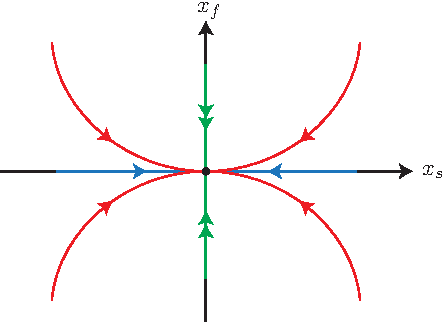
\includegraphics[width=0.4\textwidth]{figures/ch9/29simplestReduction.pdf}
	\caption{An example of the simplest setting for a nonlinear model reduction.}
	\label{fig:simplestReduction}
\end{figure}

The reduced dynamics is the same on all of these invariant manifolds, namely
\begin{align}
	\dot{x} = -ax.
\end{align}

The conclusions are similar for general $n\geq 1$ in \eqref{eq9:approx_inert_mfd} as long as $f(x) = 0$. Now we may ask ourselves if it is possible to find similar low-dimensional attracting, invariant, manifolds for $f(x) \neq 0$? To this end the simplest approach is to use linearization theorems to relate the invariant manifolds of the $f(x)=0$ case to those of the $f(x) \neq 0$ case. These come in various forms
\begin{enumerate}
	\item Hartman-Grobman theorem: If $ \textrm{Re} (\lambda_j) \neq 0$ for $j=1,\ldots,n$ then there exists a $\mathcal{C}^{0}$ linearization. However, this is insufficient for constructing smooth manifolds.
	\item Hartman theorem: If $ \textrm{Re} (\lambda_j)<0$ for $j=1,\ldots,n$ and $f\in \mathcal{C}^{2}$ then there exists a $\mathcal{C}^{1}$ linearization. This is insufficient for any Taylor expansion and does not carry over the smoothness of any manifold smoother than $\mathcal{C}^{1}$ in the linearized system.
	\item Poincaré-Dulac theorem \cite{poincare1951}: If we have $ \textrm{Re} (\lambda_j)<0$ for $j=1,\ldots,n$, $f\in \mathcal{C}^{a}$ and the following non-resonance conditions hold
		\begin{align}
			\sum_{i=1}^{n} m_i \lambda_i \neq \lambda_j;\quad \forall m\in\mathbb{N}^{n}:\ \sum_{i=1}^{n} m_{i} \geq 2
		\end{align}
		then there exists a unique $\mathcal{C}^{a}$ linearization. In this case, all invariant manifolds of the linear part of \eqref{eq9:approx_inert_mfd} continue to exist for $f(x)\neq 0$ without any change in their smoothness. It should be noted that the nonresonance condition still allows for 1:1 resonances, i.e. when $\lambda_i = \lambda_j$ for some $i,j$, but no others.
	\item Strong Sternberg linearization theorem: Under all of the conditions of the Poincaré-Dulac theorem, but for $f\in \mathcal{C}^{r}$, then there exists a $\mathcal{C}^{r}$ linearization including the case of $r=\infty $. Under nonresonance, all $\mathcal{C}^{r}$ manifolds of the linearization continue to exists for $r \in \mathbb{N}^{+}\cup \{\infty \}$.
	\item Sternberg linearization theorem \cite{Sterberg1957}: With the same non-resonance conditions as above along with $f\in\mathcal{C}^{r}$ for $r \in \mathbb{N}^{+}\cup \infty $ then there exists a $\mathcal{C}^{\rho}$ linearization where $\rho\leq r$ and $\lim_{r\to \infty }\rho = \infty $. Note that this requires no assumptions on the real parts of the eigenvalues as we had before, which means Sternberg's theorem also applies to unstable hyperbolic fixed points. In the general non-resonant case, only $f\in \mathcal{C}^{\infty }$ gives specific enough linearization that preserves the smoothness of all invariant manifolds of the linearization.  
		
\end{enumerate}
\begin{remark}[]
	Note that the nonresonance condition implies hyperbolicity of the fixed point. If there is a pair of purely imaginary eigenvalues, $\lambda=i\omega$ and $\bar{\lambda}=-i\omega$, we have, for example,
\begin{align}
\lambda + 2\bar{\lambda} = \lambda
\end{align}
and thus the nonresonance condition is violated. 
\end{remark}

In summary the results listed above guarantee that under sufficient non-resonance conditions the existence of various invariant manifolds tangent to eigenspaces even for the nonlinear system. These manifolds are called \emph{spectral submanifolds}.

We are now left with a few questions
\begin{enumerate}
	\item How do we compute spectral submanifolds in the nonlinear system?
	\item Which of the infinitely many submanifolds do we use for model reduction?
	\item As linearization of the full dynamics is more that what we need for model reduction, do such manifolds exist under less stringent conditions as well?
\end{enumerate}

To answer this we introduce the theory of (primary) spectral submanifolds and follow \cite{Ponsioen2016}. We begin by introducing the dynamical system
\begin{align}
	\dot{x} = Ax+f_0(x),\ x \in \mathbb{R}^{n},\ f_{0}(x)=\mathcal{O}\left(\|x\|^2\right),\ f_0 \in \mathcal{C}^{r},
\end{align}
for $r \in \mathbb{N}^{+}\cup\{\infty , \textrm{a} \}$ where a signifies $f_0$ being analytic. Note here that the first condition on $f_0$ implies that $x=0$ is a fixed point. The eigenvalues of $A$ given by $\lambda_1,\ldots,\lambda_n$ fulfill
\begin{align}
	\textrm{Re} (\lambda_n) \leq  \textrm{Re} (\lambda_{n-1}) \leq \ldots \leq  \textrm{Re} \lambda_1 	
\end{align}

This implies that $x=0$ is asymptotically stable. Assume that the eigenspaces are such that every eigenspace $E_j$ is the span of the real and imaginary parts of all eigenvectors and generalized eigenvectors corresponding to $\lambda_j$ for $j=1,\ldots,n$, thus we have
\begin{align}
\mathbb{R}^{n} = \bigoplus_{j=1}^{N}E_j	.
\end{align}
Such a set of eigenspaces is shown in Fig. \ref{fig:ponsioen_eigenspaces}.
\begin{figure}[h!]
	\centering
	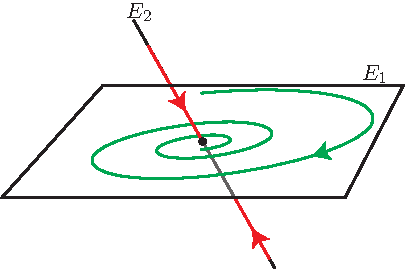
\includegraphics[width=0.6\textwidth]{figures/ch9/30ponsioen_eigenspaces.pdf}
	\caption{A set of eigenspaces fulfilling the assumption that they are generated by the eigenvectors and generalized eigenvectors.}
	\label{fig:ponsioen_eigenspaces}
\end{figure}

Next we lay out a few definitions which will be useful for studying such dynamical systems.

\begin{definition}
We call the direct sum of an arbitrary number of distinct eigenspaces the \emph{spectral subspace} 
\begin{align}
E = \bigoplus_{j=1}^{k}E_{j};\quad 1 \leq k \leq N.	
\end{align}
This always forms an invariant subspace of $\dot{x}=Ax$.
\end{definition}
\begin{definition}

The \emph{spectral quotient of $A$} is given by
\begin{align}
	\sigma(E) = \left\lfloor \frac{ \textrm{smallest Re} [\lambda _k] \textrm{ outside of }E}{ \textrm{largest Re} [\lambda _i]  \textrm{ inside of } E}\right\rfloor.
\end{align}
An illustration of these two values are given in Fig. \ref{fig:spect_quotient}.
\begin{figure}[h!]
	\centering
	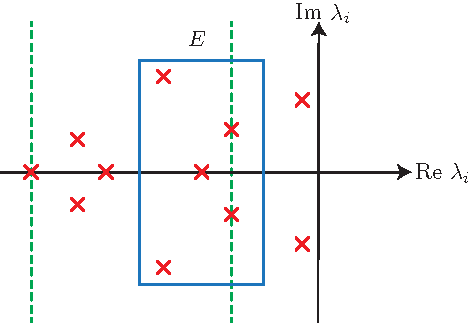
\includegraphics[width=0.6\textwidth]{figures/ch9/26spect_quot.pdf}
	\caption{The eigenvalue constellation, the left dotted green line designates the smallest real part outside of $E$ and the right dotted green line designates the largest real part inside of $E$.}
	\label{fig:spect_quotient}
\end{figure}
\end{definition}

\begin{definition}
The \emph{external non-resonance condition for $E$} with $ \textrm{dim} [E]=q$ is
\begin{align}
	\langle m, \lambda \rangle_{E} = m_1 \lambda _{j1} + \ldots + m_1 \lambda _{jq} \neq \lambda_l,\ m_i \in \mathbb{N}	,
\end{align} 
where $\lambda _{j1},\ldots,\lambda _{jq}\in  \textrm{spect}[A|_{E}] $ and $\lambda _{l} \not \in  \textrm{spect} [A|_{E}]$.
\end{definition}

We proceed by discussing the existence of a spectral subanifold (SSM) in the full nonlinear system, i.e. a nonlinear continuation of $E$. 
\begin{theorem}[]
Assume the low-order external non-resonance condition
\begin{enumerate}
	\item $\langle m, \lambda \rangle_{E} \neq \lambda _l$ for $\lambda_l \neq  \textrm{spect}[A|_{E}] $;
	\item $2 \leq |m| \leq \sigma(E)$ with the norm $|m | =m_1 + \ldots + m_1$;
\end{enumerate}
then we have that the following hold:
\begin{enumerate}
	\item There exists a $\mathcal{C}^{r}$ spectral submanifold $W(0)$ tangent to $E$ at $x=0$ with the same dimension as $E$;
	\item $W(0)$ is unique among all $\mathcal{C}^{\sigma(E) + 1}$ invariant manifolds satisfying (i);
	\item If $f_0$ is jointly $\mathcal{C}^{r}$ in $(x,\mu )$ for some parameter $\mu \in \mathbb{R}^{p}$, then so is $W(0)$, this also holds for $r=\infty $ and $r=a$. 
\end{enumerate}
Furthermore if $f_0$ is smooth or analytic in  $x$ and $\mu $, then so is $W(0)$.
\end{theorem}
\begin{proof}
	See \cite{Ponsioen2016}
\end{proof}
With this theorem, we can see that high-enough-order Taylor-series expansion puts us on $W(0)$ if we look for it as an invariant graph over $E$.

\begin{ex}[]
	Consider the dynamical system
	\begin{align}
		\begin{dcases}
			\dot{x} = - \frac{1}{4}x + xy + x^{3}\\
			\dot{y} = -y - 2x^2,
		\end{dcases}
	\end{align}
	whose dynamics is depicted in Fig. \ref{fig:SSM_ex1}.
	\begin{figure}[h!]
		\centering
		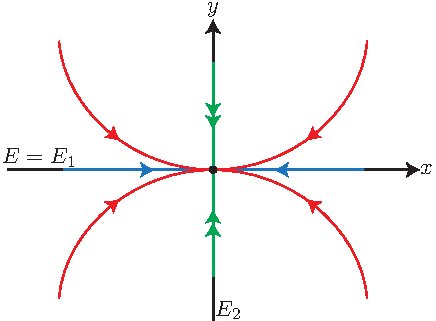
\includegraphics[width=0.6\textwidth]{figures/ch9/31ssm_ex1.pdf}
		\caption{The dynamics of the dynamical system given in the example.}
		\label{fig:SSM_ex1}
	\end{figure}	
	The slow spectral subspace is given by $E=E_1$ where $E_1$ is defined as the $x$-axis and can be seen in Fig. \ref{fig:SSM_ex1}. The spectral quotient of this manifold can be calculated as
	\begin{align}
		\sigma(E) = \left\lfloor \frac{-1}{-\frac{1}{4}} \right\rfloor = 4.
	\end{align}
	It can also be seen that $m_1$ exists such that $m_1\lambda_1 = -m_1 \frac{1}{4} = -1 = \lambda_2 $ with $2 \leq |m| =m_1 \leq 4$, namely $m_1=4$, therefore the non-resonance condition for $E$ is not fulfilled and no unique spectral submanifold as a nonlinear continuation of $E$ exists.
	Hence, we modify the system to
	\begin{align}
		\begin{dcases}
			\dot{x} = -\frac{1}{\alpha } x + xy + x^{3}\\
			\dot{y} = -y - 2x^2
		\end{dcases};\quad
		\alpha \not \in \mathbb{N}^{+} -\{1\}. \label{eq9:113}
	\end{align}
	With this modification we find that $\sigma(E) = \lfloor \alpha \rfloor$, the non-resonance condition becomes $-m_1 \frac{1}{\alpha } \neq 1$ for $2\leq m_1 \leq \lfloor \alpha \rfloor$, thus we can see why we need the restriction on $\alpha $. Assuming such an $\alpha $ we find that there exists a unique spectral submanifold in the class of $\mathcal{C}^{\lfloor \alpha \rfloor + 1}$.

	Next, we look for a spectral submanifold as a Taylor expansion over $E$. To do this write the manifold as
	\begin{align}
		y = ax^2 + bx^3 + cx^4 + \mathcal{O}(x^5) = h(x).
	\end{align}
	We can differentiate this to find
	\begin{align} 
		\dot{y} = h'(x)\dot{x} &= \left(2ax + 3bx^2 + 4cx^3 + \mathcal{O}(x^4)\right) \left( - \frac{1}{\alpha } x + xh(x) + x^3 \right) \\
				       &= -\frac{2a}{\alpha } x^2 - \frac{3b}{\alpha }x^3 - \frac{4c}{\alpha }x^4 + 2a(a+1) x^4 + \mathcal{O}(x^5). \label{eq9:uno} 
       \end{align}
       On the other hand, from equation \eqref{eq9:113} we find
       \begin{align}
		\dot{y} =\left. -y \right|_{W_E(0)} - 2x^2 &= -\left(ax^2 + bx^3 + cx^4 + \mathcal{O}(x^5)\right) - 2x^2\\
							   &= -(a+2)x^2 - bx^3 - cx^4 + \mathcal{O}(x^5). \label{eq9:dos}
	\end{align}
	By comparing \eqref{eq9:uno} and \eqref{eq9:dos} we can see
	\begin{align}
		\mathcal{O}(x^2)&:\quad \frac{2a}{\alpha } = a+2 \quad &&\implies a(2-\alpha ) = 2\alpha; \\ 
		\mathcal{O}(x^3)&:\quad \frac{3b}{\alpha } = b \quad &&\implies b(3-\alpha ) = 0;\\
		\mathcal{O}(x^4)&:\quad 2a(a+1)- \frac{4c}{\alpha }= -c \quad &&\implies c(4-\alpha )= 2a(a+1)\alpha .
	\end{align}
	These equations cannot be solved when a resonance is present. Furthermore, below order $\sigma(E)$ all manifolds have the same expansion.

We may select $\alpha =\frac{3}{2}$ which implies $\lambda_1 = -\frac{2}{3}$ and $\lambda _2 = -1$, thus we have that $a=6$, $b=0$, and $c= \frac{2a(a+1)\alpha }{\alpha -1}>0$. Hence the spectral quotient can be calculate as $\sigma(E) = \left\lfloor \frac{-1}{-\frac{2}{3}}\right\rfloor = 1$, and thus $W_E(0)$ is already unique among the class of $\mathcal{C}^{2}$ invariant manifolds. Based on this we can see that the second order Taylor expansion only exists for $W_E(0)$ 
\begin{align}
	y = 6x^2 + cx^4 + \mathcal{O}(x^5).
\end{align}
We may now write the reduced dynamics
\begin{align}
	\dot{x} = - \frac{2}{3} x + x(6x^2+cx^4 + \mathcal{O}(x^5)) + x^3 = -\frac{2}{3}x + 7x^3 + \mathcal{O}(x^4).
\end{align}
From here we derive the leading order model
\begin{align}
	\dot{x} = x\left( -\frac{2}{3} + 7x^2\right)
\end{align}
which has two nontrivial fixed points at $x = \pm \sqrt{\frac{2}{21}}$. Now we may ask if the full system has fixed points, namely by attempting to solve
\begin{align}
	\begin{dcases}
		-\frac{2}{3} x + xy + x^3 = 0\\
		-y - 2x^2 = 0.
	\end{dcases}
\end{align}
By setting the condition implied from the second equation into the first we find
\begin{align}
	-\frac{2}{3}x - x(2x^2) + x^3 = 0 \implies x\left(-\frac{2}{3} - x^2 \right) =0. 
\end{align}
This implies that no fixed point exist outside of the origin! The first order approximation of the spectral submanifold may not suffice, but we have the opportunity to go to \emph{any} order, without increasing the dimension of the reduced order model.
\end{ex}

Following the results of the previous example, we now look to extending the spectral submanifold to non-autonomous (forced) dynamical systems. For this we will assume the setup with $0\leq \varepsilon \ll 1$
\begin{align}
	\dot{x} = Ax + f_0(x) + \varepsilon f_1(x, \Omega t, \varepsilon);\quad x \in \mathbb{R}^{n},\ A \in \mathbb{R}^{n\times n},\ f_0,f_1 \in \mathcal{C}^{r},\ f_0 = \mathcal{O}(\|x\|^2).
\end{align}
Further we assume that $\Omega = (\Omega_1,\ldots,\Omega_k)\in \mathbb{R}^{k}$ has rationally independent entries and that $f_1$ is $2\pi$-periodic in the $\Omega t$ arguments. Furthermore we assume that the real parts of the eigenvalues are ascending and are all strictly less than 0, i.e. for $\varepsilon = 0$ the origin is asymptotically stable (and hyperbolic). We are interested in the spectral subspace $E= \bigoplus_{i}E_{i}$, the direct sum of eigenspaces forming a $q$ dimensional space with $q\leq n$. Expanding on the definition of the spectral quotient, let us define the absolute spectral quotient as 
\begin{align}
	\Sigma(E) = \left\lfloor \frac{ \textrm{smallest Re}(\lambda_i)  \textrm{ in spect} (A) }{ \textrm{largest Re} (\lambda _2)\textrm{ in spect} (A|_{E})} \right\rfloor
\end{align}

We may introduce the k-dimensional angle $\phi$, such that the extended phase space is given by $\mathbb{R}^{n} \times \mathbb{T}^{k}$ where the dynamics is 
\begin{align}
\begin{dcases}
	\dot{x} = Ax + f_0(x) + \varepsilon f_1(x, \phi, \varepsilon) \\
	\dot{\phi} = \Omega 
\end{dcases}
;\quad \phi = \phi_0 + \Omega(t-t_0) \in \mathbb{T}^{k}.
\end{align}
The geometry of this system for $\varepsilon=0$ is shown in Fig. \ref{fig:ssm_eps0}.
\begin{figure}[h!]
	\centering
	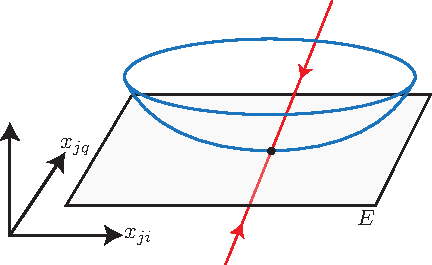
\includegraphics[width=0.6\textwidth]{figures/ch9/32ssm_ex0.pdf}
	\caption{The geometry of the $\mathbb{R}^{k}$ portion of the dynamical system with $ \textrm{dim} (E) = q$.}
	\label{fig:ssm_eps0}
\end{figure}
\begin{theorem}[]
If we have that $\langle m, \lambda \rangle_E \neq \lambda_l$ for $2 \leq |m| \leq \sigma(E)$, $\lambda_i \in  \textrm{spect} (A|_{E})$, and $\lambda_l \in  \textrm{spect} (A)- \textrm{spect} (A|_{E})$, then the following hold for $\varepsilon >0$ small enough
\begin{enumerate}
	\item There exists a unique $\mathcal{C}^{r}$ invariant torus $T_{\varepsilon}$ ;
	\item There exists a unique spectral submanifold $W_{E}(T_{\varepsilon})$ of dimension $q+k$ which is $\mathcal{O}(\varepsilon)$ $\mathcal{C}^{r}$-close to $W_{E}(0)\times T_0$;
	\item $W_{E}(T_{\varepsilon})$ is already unique among all $\mathcal{C}^{\Sigma(E) + 1}$ invariant manifolds satisfying (ii);
	\item If $f_0$ and $f_1$ are smooth or analytic, then so is $W_{E}(T_\varepsilon)$ in $\varepsilon$ too.
\end{enumerate}
\end{theorem}
\begin{remark}[]
	Note that the non-resonance condition here is stronger than that of the Theorem, and is already violated when the real part of the spectrum has an outer resonance.
\end{remark}

\begin{ex}[]
	Consider the dynamical system
	\begin{align}
		\begin{dcases}
			\dot{x} = -x \\
			\dot{y} = -\sqrt{24}y + \underbrace{x^2 + x^3 + x^4 + x^5}_{f_0} + \underbrace{\varepsilon(\sin(t) + \sin(\sqrt{2}t))}_{\varepsilon f_1}.
		\end{dcases}
	\end{align}
	Therefore we have $\Omega = (1,\sqrt{2})$, i.e. $k=2$. We have $E = E_1$ and $\Sigma(E) = \left\lfloor \frac{- \sqrt{24}}{-1}\right\rfloor = 4$, this already tells us that if it exists then $W_{E}(T_{\varepsilon})$ is unique in the smoothness class $\mathcal{C}^{5}$. Next we check that the non-resonance condition is satisfied
	\begin{align}
		\forall m_1\in\mathbb{N}^{+}: \quad m_1(-1) \neq - \sqrt{24}.
	\end{align}
	Thus we have that there exists a unique, invariant, 2 dimensional torus $T_{\varepsilon}$ which is $\mathcal{O}(\varepsilon)$ $\mathcal{C}^{r}$-close to $T_0=0\times\Pi^{2}$ and that there exists a unique spectral submanifold $W_{E}(T_{\varepsilon})$ which is 3 dimensional. Both $T_{\varepsilon}$ and $W_{E}(T_\varepsilon)$ are explicitly computable and are indeed unique in the appropriate sense. These are shown in Fig. \ref{fig:ssm_ex2}.
	\begin{figure}[h!]
		\centering
		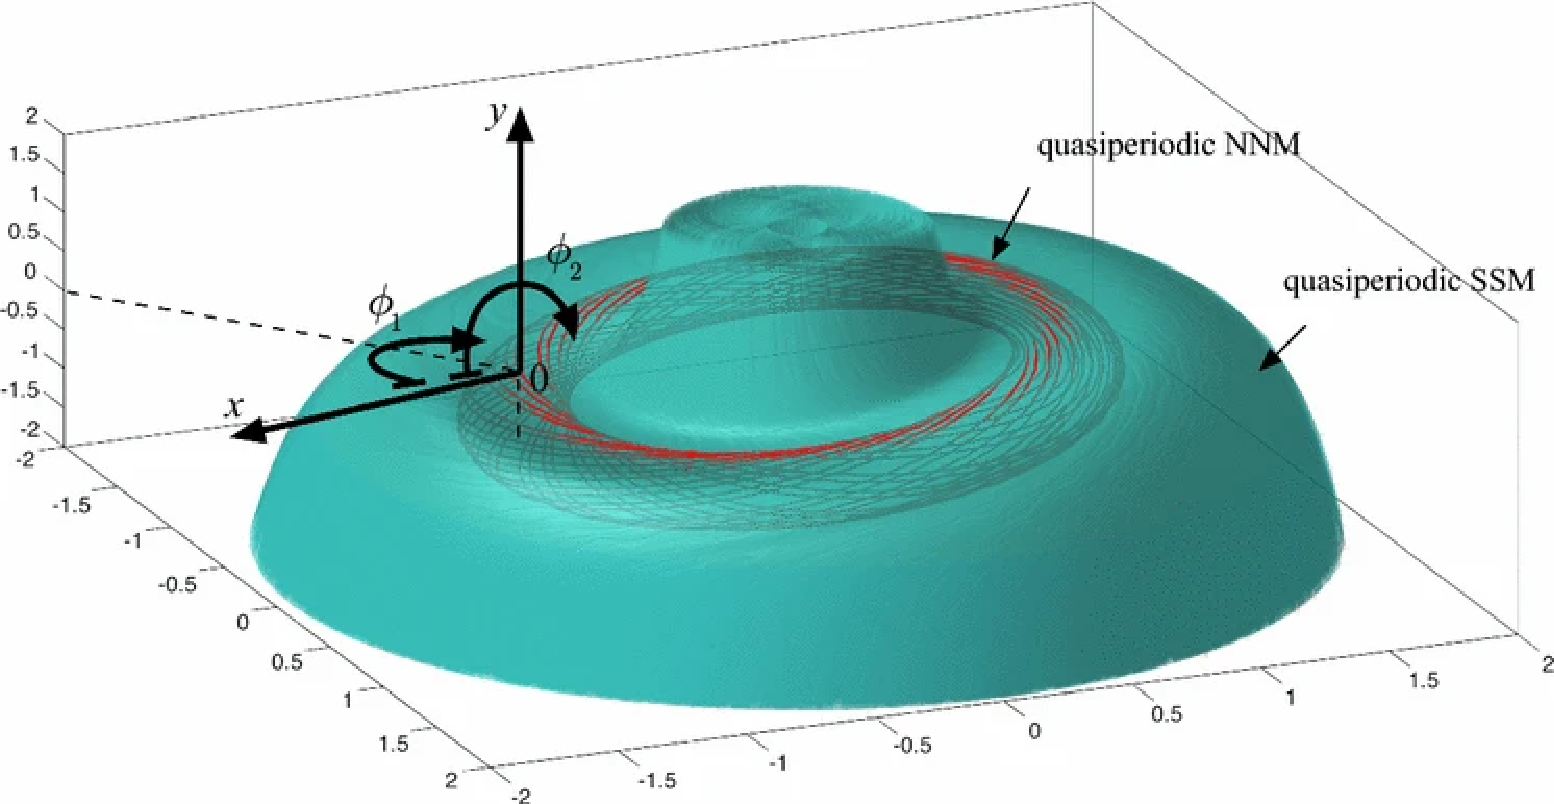
\includegraphics[width=0.8\textwidth]{figures/ch9/ponsioen2016.pdf}
		\caption{A projection of the extended phase space, the teal surface is the unique, analytic, quasiperiodic spectral submanifold, emanating from the unique quasiperiodic nonlinear normal mode in red \cite{Ponsioen2016}.}
		\label{fig:ssm_ex2}
	\end{figure}	
\end{ex}

\section{Spectral Submanifolds in Mechanical Systems}
We may now reduce the setting to mechanical systems, i.e. with $n$ degrees-of-freedom, damped-forced, weakly  nonlinear mechanical systems. Consider the dynamical system
\begin{align} \label{eq9:mech_ssm}
	M \ddot{q} + C \dot{q} + K q + N(q, \dot{q}) = \varepsilon F(q, \dot{q}, \Omega t, \varepsilon);\quad q = 
	\begin{pmatrix}
		q_1 \\ \vdots \\q_n
	\end{pmatrix} \in \mathbb{R}^{n}.
\end{align}
Again we require that $F$ is quasi-periodic in the argument $\Omega t$ with a rationally independent frequency vector $\Omega = (\Omega_1, \ldots, \Omega_k)$ with $\Omega_i\in\mathbb{R}^k$. The matrices $M$, $K$, and $C$ are all symmetric $\in \mathbb{R}^{n\times n}$ and are called the mass, stiffness, and damping matrices respectively, and all fulfill $M,K,C \succ 0$. 

The structural damping hypothesis states that $C = \alpha K + \beta M$, is convenient but is not required. Note that for $\varepsilon=0$ the eigenvalues of the linearization satisfy the characteristic equation $\det(\lambda^2 M + \lambda C + K) = 0$. This implies that $ \textrm{Re}(\lambda _{2n})\leq \ldots \leq  \textrm{Re} (\lambda _1) < 0$. For the linear system we have the ansatz $q = e^{\lambda t}A$ for $A\neq 0$. The corresponding eigensolution are the linear normal modes, written as
\begin{align}
	q_{j}(t) = \exp( \textrm{Re} (\lambda_j)t) \sin( \textrm{Im} (\lambda_j)t + \varphi_j) q_{0}^{j}.
\end{align}
The $j$-th mode shape is the constant vector $q_{0}^{j}\in \mathbb{R}^{n}$. If $ \textrm{Im} (\lambda_j) = 0$ we have an overdamped mode, otherwise if $ \textrm{Im} (\lambda _j)\neq 0$ we have an underdamped mode. The modal coordinates are 
\begin{align}
	q=Tx,\ T = ( q_{0}^{1},\ldots, q_{0}^{n})	;\quad x \in \mathbb{R}^{n}.
\end{align}
In these coordinates \eqref{eq9:mech_ssm} becomes
\begin{align}
	\ddot{x}_{i} = 2 \xi_i\omega_i \dot{x}_{i} + \omega_{i}^{2}x_i + s_i(x, \dot{x}) = \varepsilon f_i(x, \dot{x}, \Omega t, \varepsilon).
\end{align}
The natural frequency $\omega_i$ is equal to $ \textrm{Im} (\lambda_i)$ and the modal damping factor $\xi_i$ is considered overdamping if $\xi_i >1$ and underdamped if $\xi_i<1$. The modal forcing terms are contained in $f_i$. Possible nonlinear responses are shown in Fig. \ref{fig:frf}.
\begin{figure}[h!]
	\centering
	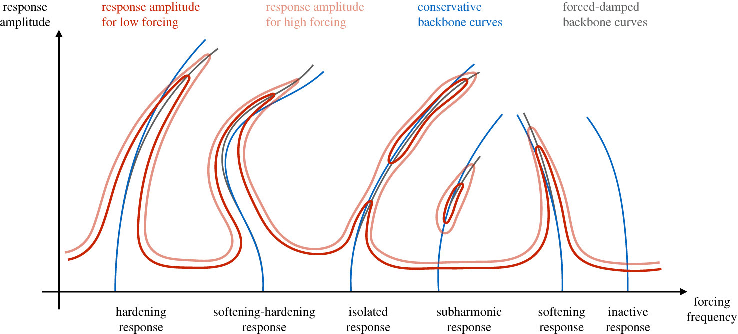
\includegraphics[width=0.99\textwidth]{figures/ch9/frf.pdf}
	\caption{Illustration of the frequency response phenomena in mechanical systems. The dark and ligh red curves identify the frequency response for low and high forcing amplitudes, respectively, while blue curves depict conservative backbone curves and grey curves represent force-damped backbone curves \cite{Cenedese_2020}.}
	\label{fig:frf}
\end{figure}

We can formulate this autonomously in the extended phase space $\mathbb{R}^{2n}\times \mathbb{T}^{k}$ 
\begin{align}
	\begin{dcases}
		\dot{x}_i = y_i \\
		\dot{y}_i = 2 \xi_i \omega_i y_i - \omega_i^2 x_i + s_i(x,y) +\varepsilon f(x,y,\phi, \varepsilon)\\
		\dot{\phi} = \Omega.
	\end{dcases}
\end{align}
The generalized quasiperiodic spectral submanifold results apply here. Note that for a typical forced response curve (e.g Fig. \ref{fig:frf}) the forcing is periodic, $k=1$. The modal subspace is the spectral subspace of the form $E=E_j$ with $E_j$ the eigenspace corresponding to the 2 eigenvalues of the $j$-th mode. Implied by the mode being overdamped, i.e. $\xi_j>1$, is that we only have negative real eigenvalues, thus the linearized dynamics on $E_j$ is described by a node. Meanwhile in the underdamped case, we have a complex conjugate pair of eigenvalues, thus the dynamics on $E_j$ is described by a stable focus.  

The modal submanifolds are the nonlinear continuations of $E_j \times \Pi^{k}$ under forcing, i.e. the spectral subbundle of perturbed invariant tori $W_{E_j}(T_{\varepsilon})$. 
%We can observe an example of the geometry in Fig. \ref{fig:ssm_ex3}.

%\begin{figure}[h!]
%	\centering
%	%\includegraphics[width=\textwidth]{}
%	\caption{An example of the geometry of a nonlinear continuation of the extended phase space.}
%	\label{fig:ssm_ex3}
%\end{figure}

Since we have the freedom to choose the dimension of the reduced order model (of the relevant spectral submanifold), this should be selected depending on how many of the transient time scales we would like to model (often stemming from the resonances with external forcing). Another consideration in this selection is that the lower-order internal resonances must be included in the spectral submanifold.

\section{System Identification with Periodic External Forcing}
The most important case in nonlinear system identification and testing is with periodic external forcing. Let us assume periodic external forcing ($k=1$, i.e. $T_0 \sim T_{\varepsilon} \sim S^1$). Our goal is to predict the forced response curve. Ideally we would find a nontrivial response near resonance which can be analyzed by reduction to $W_{E_j}(T_{\varepsilon})$. In this case $E_j$ is the modal subspace corresponding to the resonance.

The normal form for the reduced dynamics a 2 dimensional modal submanifold
\begin{align}
	\begin{dcases}
	\dot{\rho} = a(\rho) + \varepsilon (b_1(\rho, \Omega) \cos(\Psi) + b_2(\rho, \Omega)\sin(\Psi)) + \mathcal{O}(\varepsilon^2)\\
	\dot{\Psi} = b(\rho) - \Omega + \frac{\varepsilon}{\rho}(c_1(\rho, \Omega) \cos(\Psi) + c_2(\rho, \Omega)\cos(\Psi))+ \mathcal{O}(\varepsilon^2), 
\end{dcases} \label{eq9:137}
\end{align}
where we have
\begin{align}
	a(\rho) &=  \textrm{Re} (\lambda_j) + \sum_{i}^{} a_i \rho^{2i+1} \\
	b(\rho) &=  \textrm{Im} (\lambda_j) + \sum_{i}^{} b_i \rho^{2i},
\end{align}
further $b_{1,2}$ and $c_{1,2}$ in \eqref{eq9:137} are Taylor series in $\rho$, which are convergent if $W_{E_j}(T_\varepsilon)$ is analytic. We call $\rho $ the polar radius, $\Psi $ the phase lag between the polar angle $\varphi $ and phase of the forcing, i.e. $\Psi = \varphi-\Omega t$. 
\begin{theorem}[]
	Nontrivial non-spurious transverse zeros of $a(\rho)$ (at $\rho_0$) give rise to isola, created around the point $(\Omega, \rho) = (b(\rho_0), \rho_0)$.
\end{theorem}
An illustration of the time periodic spectral submanifold and isola as in the theorem are given in Fig. \ref{fig:time_periodic_ssm}.
\begin{figure}[h!]
	\centering
	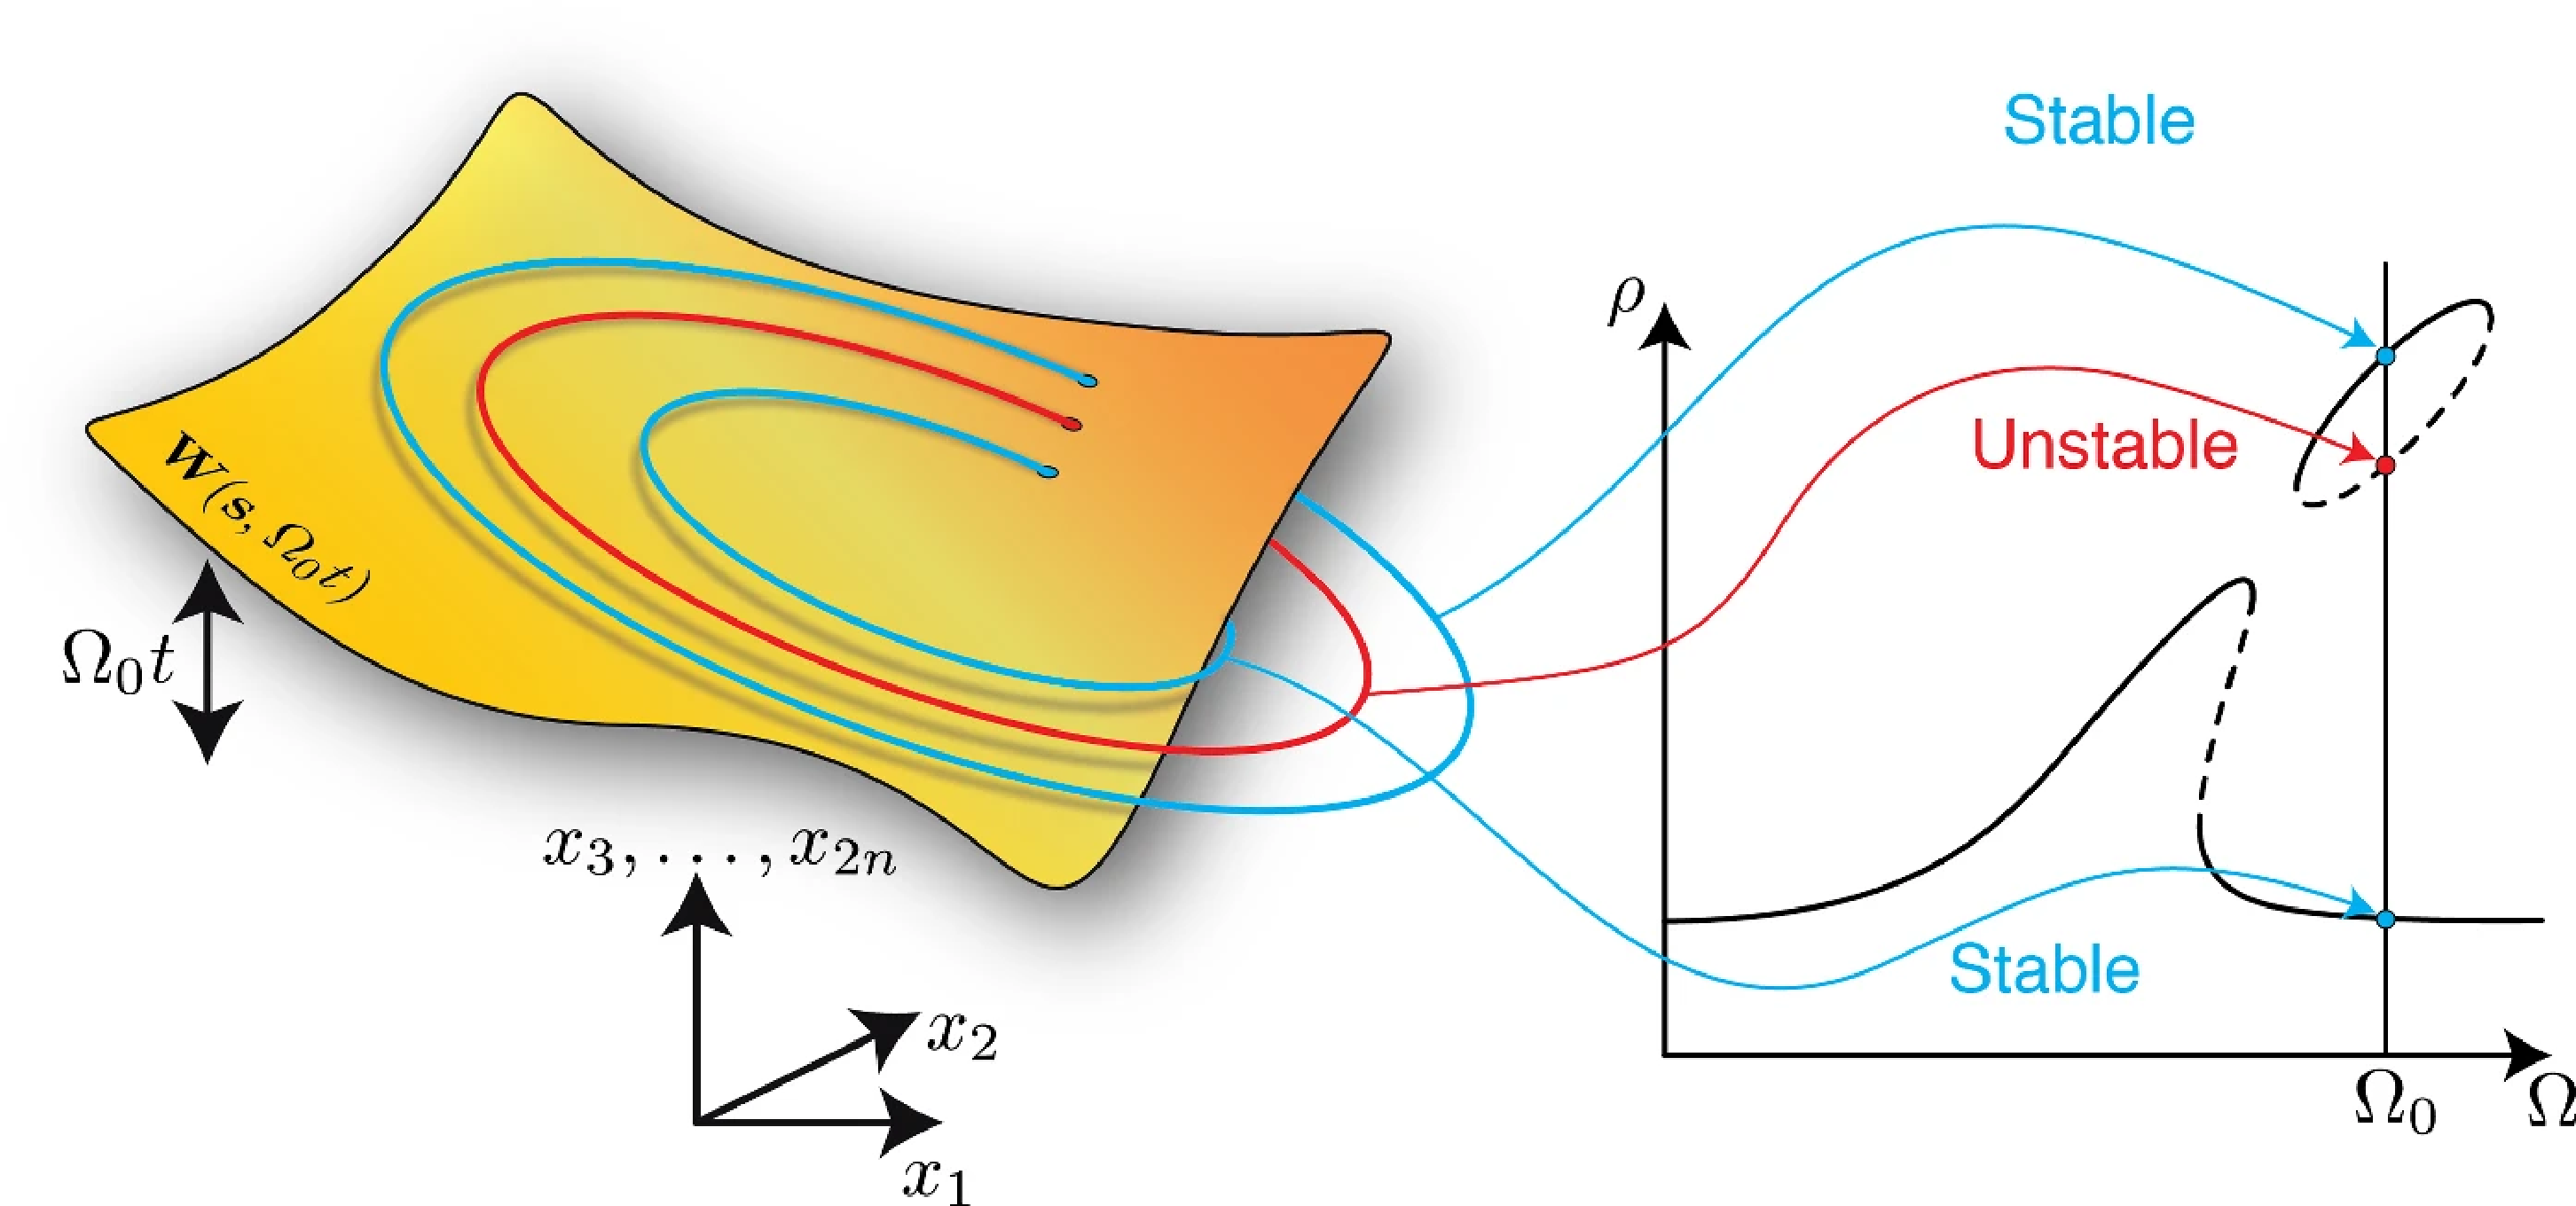
\includegraphics[width=0.6\textwidth]{figures/ch9/time_periodic_ssm.pdf}
	\caption{Illustration of a time periodic spectral submanifold. For a given forcing frequency $\Omega  $, here it is ullustrated how the spectral submanifold may contain three limit cycles, of which two fall in an isola \cite{Ponsioen2020}.}
	\label{fig:time_periodic_ssm}
\end{figure}


